\section{Experiments}
\label{sec:experiments}
In this section, we evaluated our applications based on PSWare. For each of the applications, we implemented an additional opportunistic event detection mechanism where all the events are simply transmitted to the sink for detection. The transmission is done using the existing routing protocol provided by TinyOS. This serves as reference when comparing the performance.

We compare the performance using the following metrics:
\begin{itemize}
\item Message cost: this is obtained by setting up a counter inside the sensor node. The counter will be written into flash so that we can retrieve it after the experiments.
\item Event detection delay: we measure the time between the subscription is disseminated and the event is notified.
\end{itemize}

The experimental results for the car park are shown in Figure \ref{fig:carParkResults}. In this application, we primarily consider only the message costs because the delay isn't that important in such a system. The message cost is highest during rush hour when there are a lot of cars entering and leaving the car park. To further study application uder different settings, we used two deployment strategies. The first one is even deployment, where all the parking spaces in a particular area are deployed. In the second strategy, we assume the management is only interested in a subset of the parking spaces so we randomly deployed the sensor nodes in some of the parking spaces. For all the experiments as we can see, the message cost by using application-specific middleware for ITS is the lowest while the opportunistic way is the highest.

\begin{figure}
\centering
\subfloat[With random fusion point deployment]{\label{fig:carParkResult1}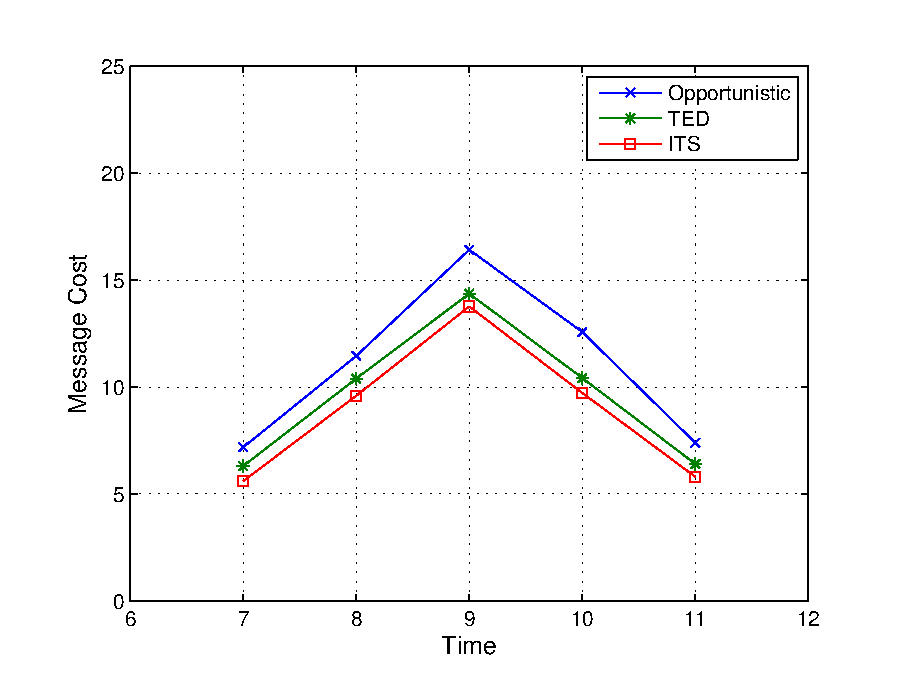
\includegraphics[width=.5\textwidth]{carParkResult1}}
%\qquad
\subfloat[With even fusion point deployment]{\label{fig:carParkResult2}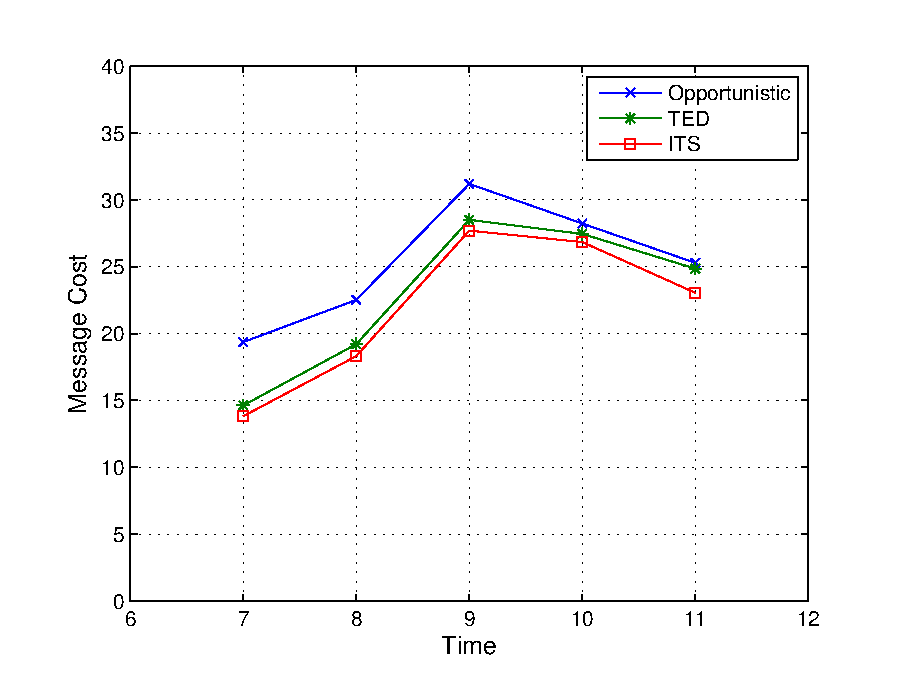
\includegraphics[width=.5\textwidth]{carParkResult2}}
\caption{Car park experiment results}
\label{fig:carParkResults}
\end{figure}

The results for ITS are shown in Figure \ref{fig:itsResults}. Different from the car park application, such applications are more delay sensitive. So we also measured the time delay for the event detection. %Similar to the car park application, ITS-specific event detection mechanism can save most energy. Both ITS and TED will introduce certain amount of delay due to the waiting.
 
\begin{figure}
\centering
\subfloat[Message cost]{\label{fig:itsResult1}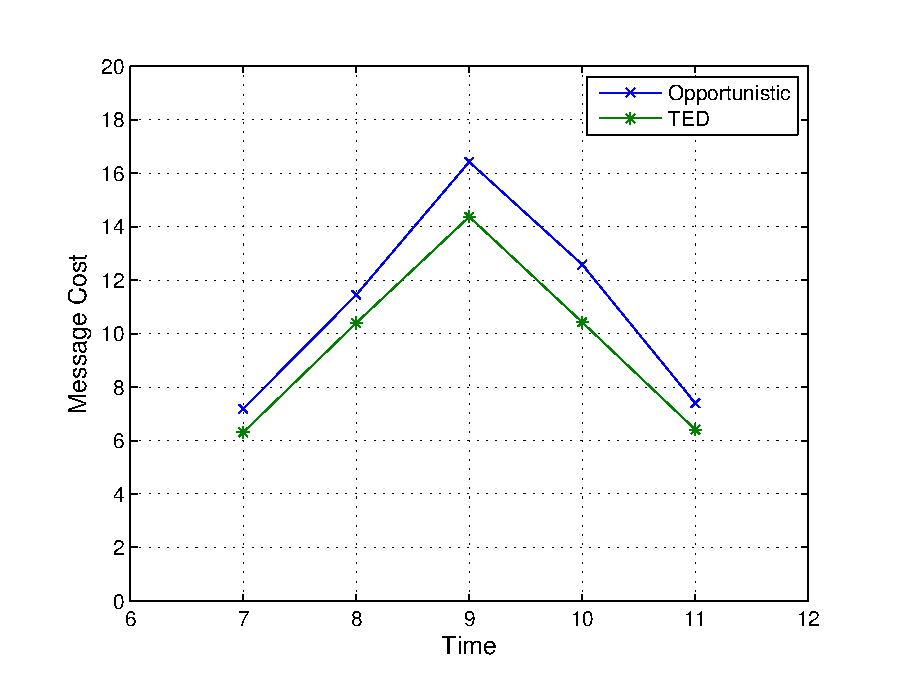
\includegraphics[width=.5\textwidth]{itsResult1}}
%\qquad
\subfloat[Delay]{\label{fig:itsResult2}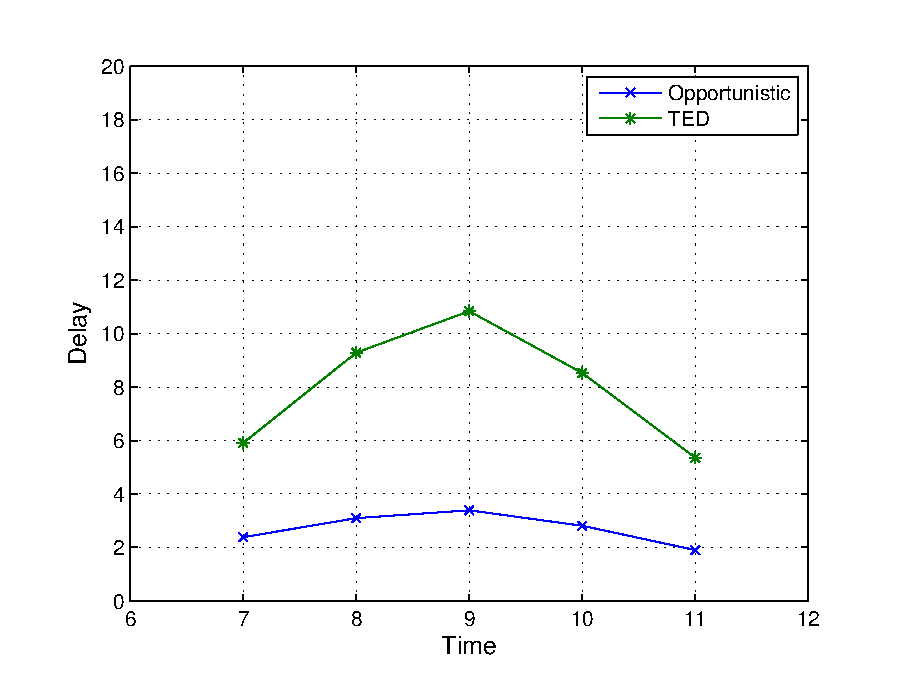
\includegraphics[width=.5\textwidth]{itsResult2}}
\caption{Experiments on the roads}
\label{fig:itsResults}
\end{figure}

Our final experiments is for indoor monitoring. We consider the application scenario where the sensor nodes are deployed in a building so that the temperature can be monitored. As discussed in the previous sections, such an application can probably be useful for certain types of context aware pervasive applications such as indoor temperature monitoring. The experimental results is shown in Figure \ref{fig:itsResults}. 

\begin{figure}
\centering
\subfloat[With random fusion point deployment]{\label{fig:indoorResult1}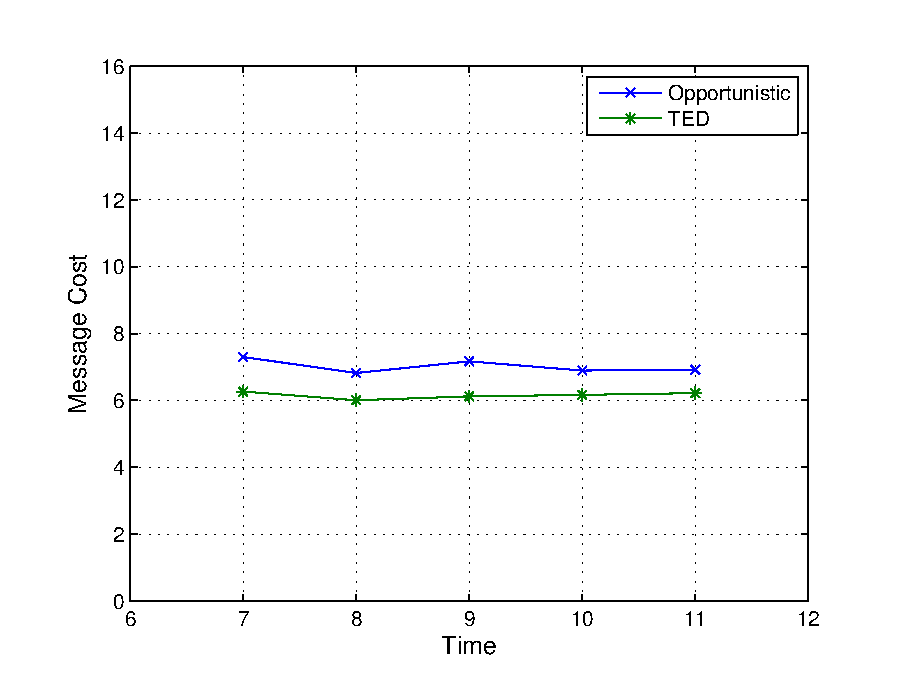
\includegraphics[width=.5\textwidth]{indoorResult1}}
%\qquad
\subfloat[With even fusion point deployment]{\label{fig:indoorResult2}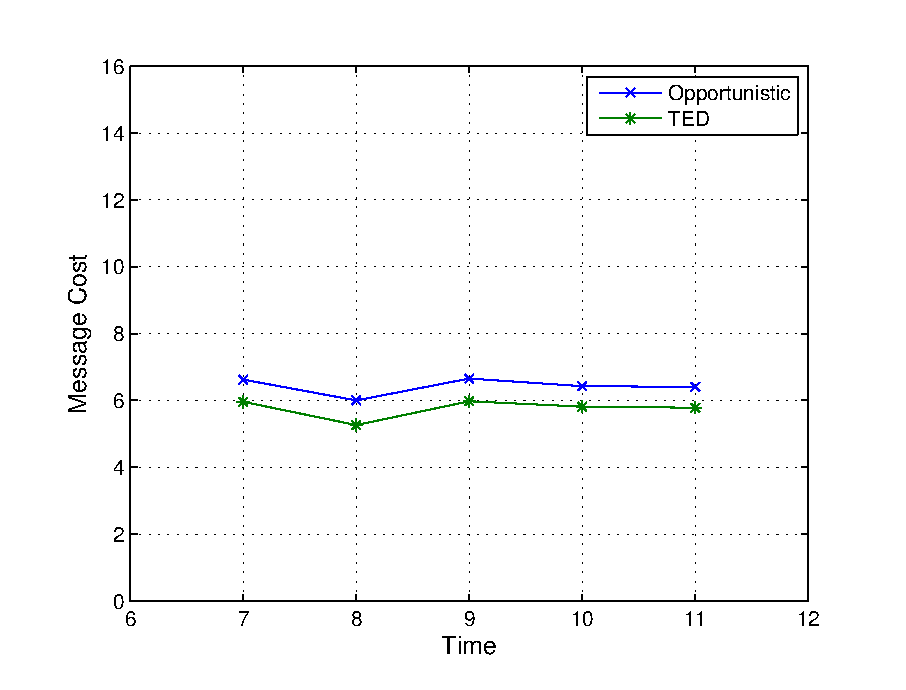
\includegraphics[width=.5\textwidth]{indoorResult2}}
\caption{Experiments for temperature monitoring}
\label{fig:indoorResult}
\end{figure}